\chapter{Mission} % <<< ---------------------------------------------------------------------------------
\label{ch:mission}
% ---------------------------------------------------------------------------- %

This chapter presents a brief summary of the hardware platform and some of its
key characteristics  which are of  interest to us. From that  information, the
objectives of  this project  are derived. Possible  approaches to  reach those
objectives are  presented and evaluated, and  a decision is reached  on how to
achieve this project's aims. At the end  of this chapter, the reader will know
what we intend to do and why.


\section{The Red Pitaya STEMlab 125-14} % <<< -------------------------------- %
\label{sec:stl125}
% ---------------------------------------------------------------------------- %

First, some key  specifications of the hardware are given,  to then proceed to
the key problems which occur when downsampling with its stock configuration.


\subsection{Hardware Overview} %<<< ------------------------------------------ %
\label{subsec:stl125:hardware_overview}
% ---------------------------------------------------------------------------- %

The  device on  which this  project  is based  is the  Pitaya STEMlab  125-14,
pictured  in Figure~\ref{fig:stl125:photo}. STEMlab  is a  compact measurement
instrument (it fits into the palm of  a hand) which can replace more expensive
devices like  oscilloscopes by using  a computer for data  storage, processing
and presentation.

Some of its key specifications relevant to us are:
\begin{itemize}\tightlist
    \item
        two high-speed analog inputs and outputs via coaxial connectors
    \item
        Uses  a  Linear Technology  LTC2145-14  converter~\cite{lt:ltc2145-14}
        on      those      inputs:      \num{14}\,bits      resolution      at
        \num{125}\,MS$\cdot$s\textsuperscript{-1} per channel.
    \item
        Xylinx SOC  with an FPGA component  for data processing on  the device
        itself and two ARM Cortex9 chips for general-purpose tasks
    \item
        Ethernet and USB connections for data transmission and device control
    \item
        Has its own operating system, a GNU/Linux distribution (Ubuntu is used
        in our project), running on the ARM cores.
    \item
        The software used is open-source and available under \cite{pita:github}.
\end{itemize}
More  comprehensive documentation  can be  found at~\cite{pita:readthedocs}. A
block   diagram   with    the   system's   key   components    is   shown   in
Figure~\ref{fig:stl125:block_diagram}.

\begin{figure}
    \centering
    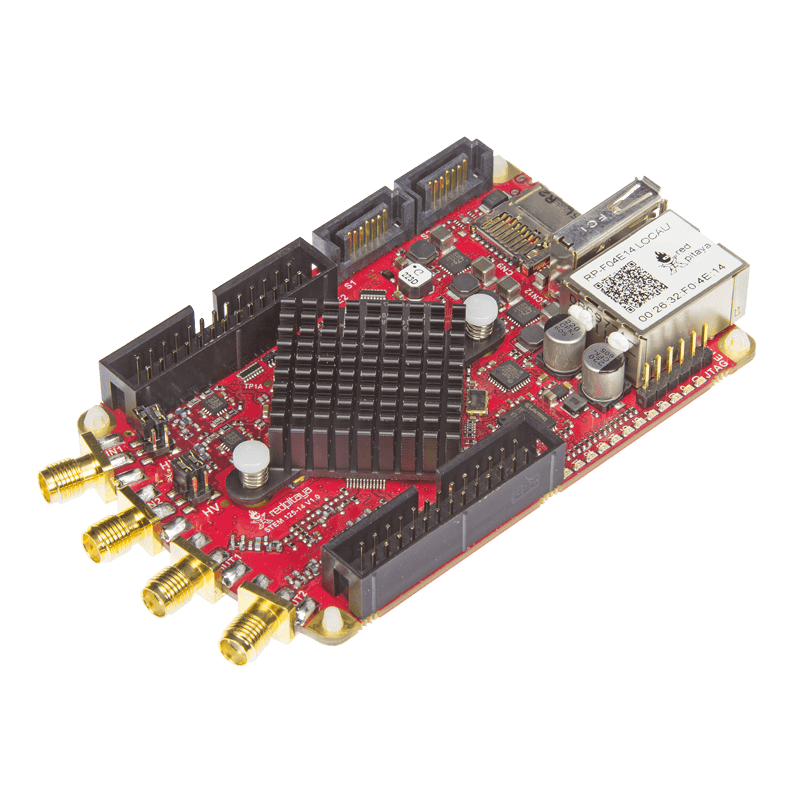
\includegraphics[width=0.67\textwidth]{images/stl125/stemlab125-14-photo.png}
    \caption{Block diagram of the Red Pitaya STEMlab. Source:~\cite{pita:elektor:starterkit}}
    \label{fig:stl125:photo}
\end{figure}

\begin{figure}
    \centering
    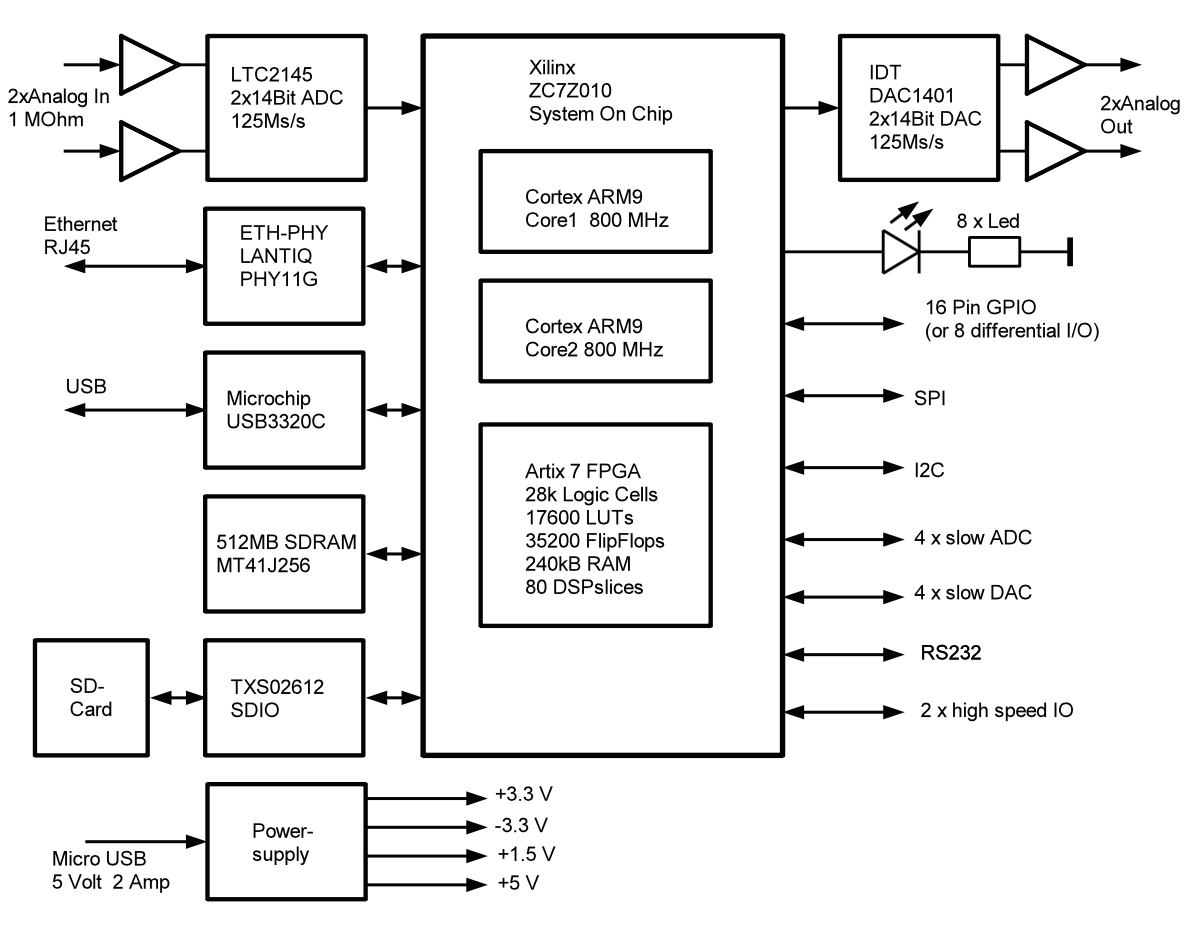
\includegraphics[width=\textwidth]{images/stl125/stemlab125.png}
    \caption{Block diagram of the Red Pitaya STEMlab. Source:~\cite{pita:ossmann}}
    \label{fig:stl125:block_diagram}
\end{figure}
%>>>


\subsection{Downsampling on the STEMlab With Stock Configuration} %<<< ------- %
\label{subsec:stl125:ds_default}
% ---------------------------------------------------------------------------- %

The  STEMlab  enables   downsampling  by  powers  of  \num{2}   in  its  stock
configuration, in a range  between $1 = 2^0$ and $65536  = 2^{16}$.  The exact
manner in which this downsampling process is performed is not easily deducible
from  public information;  the  documentation  on the  internals  of the  FPGA
codebase  is  rather  sparse. However,  work  conducted  by  our  predecessors
has  shown  that  the  STEMlab  uses   a  moving  averaging  filter  for  this
process~\cite{bucher:kuery}.

The moving averager's transfer function is
\begin{equation}
    \label{eq:moving_averager}
    H(z) = \frac{1}{N+1}\sum_{k = 0}^{N} z^{-k}.
\end{equation}
A high degree of similarity is immediately recognizable when comparing this to
the  transfer  function  of  a CIC  filter  in  Equation~\ref{eq:cic:complete}
(page~\pageref{eq:cic:complete}). Indeed, a cascade  of moving averagers would
almost yield a CIC  filter, save for the gain, which  could be easily adjusted
after the fact if needed.

A moving averager as a decimation filter is relatively cheap to implement when
using only  decimation rates of powers  of two, as  is the case for  the stock
software of the  STEMlab. The weight for each coefficient of  $z^{-k}$ will be
$\frac{1}{N+1}  =  \frac{1}{R} =  2^{-m},  m  \in \mathbb{N}_0$,  meaning  the
computations can  be performed without  multipliers by performing  a bit-shift
operations to  the right. The  primary disadvantage  which results  from these
rate reduction  factors is that the  resulting reduced sampling rates  are not
very  ``nice'' numbers,  so  to speak,  since the  incoming  sampling rate  is
\SI{125}{\MHz}, and therefore not a power of \num{2}.

Just  like a  CIC filter  by  itself, however,  a moving  averager also  makes
for  a  rather  poor  lowpass  filter, for  two  reasons: Passband  droop  and
poor  stopband   attenuation  (equivalent  to  a   single-stage  CIC  filter).
Figure~\ref{fig:stl125:moving_averager} shows  the frequency response  for the
case of  $R=8$ and  a signal  of \SI{5}{\MHz}. The  incoming sampling  rate is
\SI{125}{\MHz},  the  reduced  sampling  rate  is  $\SI{125}{\MHz}  \div  8  =
\SI{15.625}{\MHz}$. Therefore, anything  above half that frequency  is aliased
back into the region below $\SI{15.625}{\MHz} \div 2 = \SI{7.8125}{\MHz}$.  In
the case of a signal at  \SI{5}{\MHz}, this results in an aliasing attenuation
of a paltry \SI{8.06}{\dB}. Combined with the passband droop of \SI{1.48}{\dB}
(a signal  attenuation of  almost \SI{16}{\percent})  at that  frequency, this
makes for a  margin of a mere \SI{6.58}{\dB} between  the signal's attenuation
and the aliasing attenuation!

\begin{figure}
    \centering
    \newcommand*\freqzFileMAA{images/stl125/movingAveragerPBAliasingComplete.csv}
\newcommand*\freqzFileMAB{images/stl125/movingAveragerPBAliasingNull1Left.csv}
\newcommand*\freqzFileMAC{images/stl125/movingAveragerPBAliasingNull1Right.csv}
\newcommand*\freqzFileMAD{images/stl125/movingAveragerPBAliasingNull2Left.csv}
\newcommand*\freqzFileMAE{images/stl125/movingAveragerPBAliasingNull2Right.csv}
\newcommand*\freqzFileMAF{images/stl125/movingAveragerPBAliasingNull3Left.csv}
\newcommand*\freqzFileMAG{images/stl125/movingAveragerPBAliasingNull3Right.csv}
\newcommand*\freqzFileMAH{images/stl125/movingAveragerPBAliasingNull4Left.csv}
\pgfplotstableread[col sep=comma]{\freqzFileMAA}\freqzTableMAA
\pgfplotstableread[col sep=comma]{\freqzFileMAB}\freqzTableMAB
\pgfplotstableread[col sep=comma]{\freqzFileMAC}\freqzTableMAC
\pgfplotstableread[col sep=comma]{\freqzFileMAD}\freqzTableMAD
\pgfplotstableread[col sep=comma]{\freqzFileMAE}\freqzTableMAE
\pgfplotstableread[col sep=comma]{\freqzFileMAF}\freqzTableMAF
\pgfplotstableread[col sep=comma]{\freqzFileMAG}\freqzTableMAG
\pgfplotstableread[col sep=comma]{\freqzFileMAH}\freqzTableMAH
\begin{tikzpicture}
     \pgfplotsset{every axis/.style={
            height=140mm,
            width=\textwidth,
            grid=none,
            y filter/.code={\pgfmathparse{20*log10(\pgfmathresult))}},
            x filter/.code={\pgfmathparse{\pgfmathresult / 3.141592654}},
            x SI prefix=mega,
            x unit=\si{Hz},
            xticklabel style={font=\footnotesize},
            y unit=\si{dB},
            xlabel=Frequency,
            ylabel=Magnitude,
            xticklabel style={rotate=90},
            xmajorgrids=true,
        },
    }
    \begin{axis}[
            title=Passband Aliasing for Moving Averager,
            at = {(0,0)},
            xmin=0.001,
            xmax=1,
            ymin=-60,
            ymax=5,
            xtick={
                0,
                0.08,
                0.125,
                0.25,
                1%
            },
            xticklabels={%
                $0$,
                $f_\mathrm{signal} = \SI{5}{\MHz}$,
                $f_\mathrm{s,low}/2  = \SI{7.8125}{\MHz}$,
                $f_\mathrm{s,low}  = \SI{15.625}{\MHz}$,
                $f_\mathrm{s,high}/2 = \SI{62.5}{\MHz}$%
            },
            ytick={
                0,
                -20,
                -40,
                -60%
            },
        ]
        % Aliasing rectangles
        \fill[q0,opacity=0.20] ($(0.25*0.75,     -8.0571)$) rectangle ($(0.25*1.00,-60)$);
        \fill[q1,opacity=0.20] ($(0.25*1.00,     -8.0571)$) rectangle ($(0.25*1.25,-60)$);
        \fill[q2,opacity=0.20] ($(0.50-0.25*0.25,-8.0571)$) rectangle ($(0.50+0.25*0.00,-60)$);
        \fill[q3,opacity=0.20] ($(0.50-0.25*0.00,-8.0571)$) rectangle ($(0.50+0.25*0.25,-60)$);
        \fill[q4,opacity=0.20] ($(0.75-0.25*0.25,-8.0571)$) rectangle ($(0.75+0.25*0.00,-60)$);
        \fill[q5,opacity=0.20] ($(0.75-0.25*0.00,-8.0571)$) rectangle ($(0.75+0.25*0.25,-60)$);
        \fill[q6,opacity=0.20] ($(1.00-0.25*0.25,-8.0571)$) rectangle ($(1.00+0.25*0.00,-60)$);

        % Signal Frequency
        \draw[very thick,q5] (0.08,-60) -- (0.08,5);

        % Matlab results (copied by hand from movingAverager.m's output
        % aliasing_max_db         = -8.057121813367473 
        % passband_droop_db       = -1.475566945544402 
        % aliasing_attenuation_db =  6.581554867823072
        \draw (0, 0)      -- (0.47, 0);
        \draw (0,-1.4756) -- (0.47,-1.4756);
        \draw (0,-8.0571) -- (0.35,-8.0571);
        \draw[latex-latex] (0.34,-1.4756) -- (0.34,-8.0571);
        \draw[-latex]      (0.46, 0.5) -- (0.46, 0);
        \draw[-latex]      (0.46,-2)   -- (0.46,-1.4756);
        \draw              (0.46,0)    -- (0.46,-1.4756);
        \node[anchor=east] 
            at (0.825,-0.735)
            {\footnotesize passband droop at $f_\mathrm{signal}$: \SI{1.48}{\dB}};
        \node[anchor=east] 
            at (0.825,-4.9914) 
            {\footnotesize signal to aliasing attenuation at $f_\mathrm{signal}$: \SI{6.58}{\dB}};

        \addplot[very thick,da1,-] table[x=w, y=abs(H)] \freqzTableMAA;
        \addplot[line cap=round,very thick,q0,-] table[x=w, y=abs(H)] \freqzTableMAB;
        \addplot[line cap=round,very thick,q1,-] table[x=w, y=abs(H)] \freqzTableMAC;
        \addplot[line cap=round,very thick,q2,-] table[x=w, y=abs(H)] \freqzTableMAD;
        \addplot[line cap=round,very thick,q3,-] table[x=w, y=abs(H)] \freqzTableMAE;
        \addplot[line cap=round,very thick,q4,-] table[x=w, y=abs(H)] \freqzTableMAF;
        \addplot[line cap=round,very thick,q5,-] table[x=w, y=abs(H)] \freqzTableMAG;
        \addplot[line cap=round,very thick,q6,-] table[x=w, y=abs(H)] \freqzTableMAH;
    \end{axis}
\end{tikzpicture}

    \caption{%
        Frequency  response, passband  droop  and aliasing  attenuation for  a
        moving  average  filter  of  order  \num{7}  for  a  decimation  by  a
        factor of \num{8}. The incoming  sampling frequency is \SI{125}{\MHz},
        the  outgoing sampling  frequency is  \SI{15.625}{\MHz}, the  measured
        signal  has   a  frequency   of  \SI{5}{MHz}.%
    }
    \label{fig:stl125:moving_averager}
\end{figure}

As  a benchmark  for  or  own solution,  we  will  use measurements  conducted
by  our  predecessors  with  the  STEMlab's  stock  configuration,  listed  in
Table~\ref{tab:stl125:measurements_bucher_kuery}. The   measurements  do   not
actually  suggest  a very  bad  performance  of  the filter. This  is  because
they   were   conducted   at  specific   harmonic   frequencies. The   primary
issue  with  a   moving  averager  is  less  SNR   for  specific  frequencies,
but  aliasing  when  measuring  a  non-harmonic  signal  which  has  frequency
components above  $f_\mathrm{s,low}/2$. In that case, the  considerations from
Figure~\ref{fig:stl125:moving_averager}  become crucial  to understanding  the
aliasing issue.  This behavior was also confirmed in~\cite{bucher:kuery}.  Our
primary aim  is therefore more  to reduce  these aliasing effects  rather than
purely trying to improve SNR for specific single frequencies.

\begin{table}
    \centering
    \caption{%
        Measurement results  for STEMlab  125-14 from~\cite{bucher:kuery}. SNR
        was  determined for  a  specific harmonic  frequency  signal for  each
        sampling rate.%
    }
    \label{tab:stl125:measurements_bucher_kuery}
    \begin{tabular}{>{$}r<{$}>{$}r<{$}>{$}r<{$}SSS}
        \toprule
        R      &   &       & {$f_\mathrm{s,low}$ (\si{\kHz})} & {$f_\mathrm{signal}$ (\si{\kHz})} & SNR \\
        \midrule
        2^0    & = &     1 & 125000     & 10000   & \SI{62.8}{\dB} \\
        2^3    & = &     8 &  15625     &  5000   & \SI{69.8}{\dB} \\
        2^6    & = &    64 &   1953     &   500   & \SI{76.0}{\dB} \\
        2^{10} & = &  1024 &    122.1   &    40   & \SI{76.4}{\dB} \\
        2^{13} & = &  8192 &     15.26  &     5   & \SI{82.4}{\dB} \\
        2^{16} & = & 65536 &      1.907 &     0.5 & \SI{83.5}{\dB} \\
        \bottomrule
    \end{tabular}
\end{table}

In conclusion, we can formulate three main objectives:
\begin{itemize}
    \item
        Reduce  aliasing   of  out-of-range  frequency  components   into  the
        passband.
    \item
        Improve SNR.
    \item
        Have a nicer set of reduced sampling rates.
\end{itemize}

%>>>

%>>>


\section{Possible Solutions} % <<< ------------------------------------------- %
\label{sec:mission:possible_solutions}
% ---------------------------------------------------------------------------- %

Based on the  previous section, it is clear that  the downsampling filter from
the  STEMlab's  stock  configuration  must  be  replaced  if  better  aliasing
attenuation is  to be attained. Furthermore,  since a new filtering  system is
being implemented  anyway, one may wish  to change the rate  change factors in
order to achieve  a set of nicer-looking reduced  sampling rates. The question
now becomes: \emph{How}?

Problematic is that  as of spring 2017,  the official code by  Red Pitaya base
has been  split into  two: There is  a new  development branch  bringing major
changes, while  the old code  (which has been  used in the  projects preceding
this one) is no longer being maintained, as explained by one of the developers
(see~\cite{pita:github:issue:huesser:jeras}):
\begin{quote}
    Current  development  is done  on  the  \code{mercury} branch  on  the
    FPGA  subproject of  the same  name.  The  code is  still under  heavy
    development and  not stable. All  other FPGA  subprojects will  not be
    developed further.
\end{quote}

Essentially, this presents us with three options on how to proceed:
\begin{itemize}
    \item
        Use  the old  Red Pitaya  codebase,  and implement  our new  filtering
        system based  on that.
    \item
        Use the new  Red Pitaya codebase. Due to this  codebase being unstable
        according to the developers themselves as of the time of this project,
        we consider this to be an unviable option.
    \item
        Use an alternative  ecosystem, either by a third party  (if one can be
        found) or developed by ourselves.
\end{itemize}
In   order    to   have    a   somewhat    objective   measure    to   compare
the   first   and   last   option,    a   decision   matrix   is   used;   see
table~\ref{tab:decision_matrix:pitaya_vs_own}. In  the  following  paragraphs,
the criteria and weighings in the  table are elaborated upon. The table uses a
scale of  \num{1} through \num{6},  with \num{1}  being the worst  and \num{6}
being the best score. At the end, totals are tallied and compared.

\paragraph{Reliance  upon others:} Using  the  existing  Red Pitaya  ecosystem
would also  couple us  to any problems  inherent to that  platform and  to the
solutions developed by preceding projects based on it. Any bugs encountered in
the Red Pitaya ecosystem would either  require a bugfix by the manufacturer or
a workaround on our part. Since the old Red Pitaya codebase is no longer being
maintained by  the developers, bugfixes will  not be available, leaving  us to
clean  up  any potential  issues  inherent  to  the  codebase. If we  were  to
implement our  own solution instead, we  would be less reliant  upon others to
fix  any inherent  problems to  the code. These  factors lead  us to  give the
existing codebase a rather weak rating of, compared to a strong rating for the
choice of pursuing our own solution.

\paragraph{Flexibility:} Obviously, implementing our own  system would give us
much higher flexibility  than using the existing ecosystem. The  only two true
limitations would  be the  time and  hardware resources  available to  us. the
official codebase would limit us to its capabilities. Adding new functionality
to the existing codebase would be possible, but adapting software for purposes
for which  it was  not originally  intended does tend  to be  a time-consuming
procedure  in our  experience.  Therefore,  the option  of developing  our own
solution wins out again here.

\paragraph{Complexity  of  complete  system:} This  refers  not  just  to  the
complexity  of  the  components  we  work  on,  but  of  the  entire  platform
and  ecosystem. As  anyone who  bothers  to  peruse  the Red  Pitaya  codebase
(\cite{pita:github}) can  dedude, it is  a large ecosystem with  many features
and capabilities, most of which are not relevant to our needs. A custom system
developed for the specific needs of this project would be much leaner and have
fewer points of failure.

\paragraph{Labor  costs:} Here  is where  using  the  existing codebase  would
be  beneficial  in our  view. While  understanding  its inner  workings  would
doubtlessly be required and take a significant amount of time (particularly in
view  of  the sparse  documentation  at  this  point  in time),  developing  a
completely  new system  more or  less from  scratch would  be a  much costlier
undertaking in terms of required man-hours, we estimate.

\paragraph{Chances of success:} Basing our work on the existing codebase would
unburden  us  of  the  legwork  needed  to  get  basic  functionality  up  and
running. We could exchange  the filter components of the  existing system with
our own, but leave most of the remaining system untouched. The challenge would
be to understand the  system well enough to do this.   Building our own system
would require re-implementing more components  of the Red Pitaya platform than
just the filters. As each additional task  increases the risk of failure, this
is not without  risk to the overall success. Overall, we  consider this factor
to be roughly even between the two choices.

\paragraph{Robustness  of third-party  components:} This criterion  takes into
account our assessment  of the reliability and dependability  of any component
we use which  is not developed by ourselves, along  with its documentation and
manufacturer  support. In the  case of  the  Red Pitaya  codebase, this  would
primarily  comprise the  codebase  itself as  well as  any  components for  it
developed  by other  parties. If  we were  to develop  our  own solution,  the
building blocks would primarily be the  Xilinx toolchain and libraries for the
SoC.

Because  the  Red  Pitaya  codebase  is rather  large,  not  well  documented,
comparatively new and no longer being maintained, and the company is small and
more likely  to be  stretched thin, we  do not score  the Red  Pitaya codebase
highly here. The  Xilinx toolchain and  FPGA libraries, while  undoubtedly not
without bugs,  have had  a lot  of time to  mature on  the other  hand.  Also,
Xilinx is a big company with vast resources, so any bugs which are encountered
in  their products  are more  likely to  be addressed  in our  view. For these
reasons, we score  developing our own solution higher than  using the existing
cosebase.

\paragraph{Reparability:} If any issues are found in the resulting product, we
are more likely to  be able to fix them if it is  our own codebase rather than
that by a third party.

\paragraph{Long-term viability:} Developing  our own  solution would  allow us
(or anyone  else wishing  to base their  work off of  ours) to  address future
needs relatively  easily. Using the  existing code base  would make  this more
difficult in our view.

\paragraph{Conclusion:} Developing our  own solution does carry  a significant
risk  and is  likely  to require  more  work than  basing  our application  on
existing  work.   But in  light  of  the  mentioned  drawbacks of  the  latter
approach, we still find that it is  the preferable approach and is more likely
to lead to a successful outcome.


\begin{table}
    \centering
    \caption{%
        Decision   matrix   comparing   the   usage  of   the   existing   Red
        Pitaya   ecosystem  against   building   our   own  data   acquisition
        system. Weighing: Scale  of \num{1}  (worst)  to \num{6}  (best). More
        total points is better.%
    }
    \label{tab:decision_matrix:pitaya_vs_own}
    \begin{tabular}{>{\raggedright}p{80mm}SS}
        \toprule
        & RP & Custom \\
        \midrule
        reliance on others &
        2 & 5 \\

        flexibility &
        2 & 5 \\

        complexity of complete system &
        1 & 4 \\

        labor costs &
        4 & 2 \\

        chances of success &
        4 & 4 \\

        available documentation for used building blocks &
        3 & 5 \\

        robustness of third-party components &
        2 & 5 \\

        reparability &
        2 & 5 \\

        long-term viability&
        2 & 4 \\
        \midrule
        Total & 21 & 37 \\
        \bottomrule
    \end{tabular}
\end{table}

%>>>


\section{Concept} % <<< ------------------------------------------------------ %
\label{sec:mission:concept}
% ---------------------------------------------------------------------------- %

Having concluded that  we shall develop our own solution  from scratch, we can
now  develop  a  concept  for  how  that solution  will  look.   On  the  most
fundamental level, it will require the following components:
\begin{itemize}
    \item
        a custom FPGA firmare for data acquisition and filtering
    \item
        a new scope application for data visualization
    \item
        an interfacing layer between the FPGA and the scope
    \item
        optionally, the possibility to connect to other applications like Matlab
\end{itemize}
The   following   sections   elaborates   on  the   general   shape   of   our
solution. Chapters~\ref{ch:fpga}  through~\ref{ch:graphical_front_end} explain
the components  in detail, while Chapter~\ref{ch:filter_design}  documents the
filter design process, which is rather separate from the firmware and software
and therefore a dedicated chapter.


\subsection{FPGA Components} % <<< ------------------------------------------- %
\label{subsec:concept:fpga_components}
% ---------------------------------------------------------------------------- %

On the most abstract level, the FPGA part of our system will need to be able to
\begin{itemize}\tightlist
    \item
        acquire data from the ADC,
    \item
        decimate and filter it,
    \item
        and pass it on for further processing.
\end{itemize}

Due to the  platform's open nature, there exist some  projects for the STEMlab
by parties other than Red Pitaya  themselves. One of these is \emph{Red Pitaya
Notes} by  Pavel Denim, available  at~\cite{pita:github:pitaya-notes}. As part
of that  project, Mr. Denim  has implemented  an ADC core  for the  FPGA which
acquires  data from  the ADC's  two  channels and  passes  it on  via an  AXI4
streaming interface\footnotemark.
\footnotetext{%
    Xilinx's proprietary general-purpose interconnect for moving large amounts
    of data around an FPGA
}
Since   this   project  is   open-source   and   has  a   permissive   license
(MIT   license~\cite{licenses:mit},   template   text    can   be   found   in
Appendix~\ref{sec:mit_license} on page~\pageref{sec:mit_license}) and fulfills
our  main technical  requirement (easily  interfaceable),  it is  used in  our
project to interface the FPGA with the ADC.

For filtering,  one can either  implement custom filter topologies  from basic
FPGA building blocks (adders, multipliers, etc.), write completely custom VHDL
or Verilog code, or use ready-made blocks, if available.  Xilinx provides such
FPGA  blocks for  FIR  and CIC  filters,  both of  which  come with  excellent
documentation  (see~\cite{xilinx:cic-compiler} and~\cite{xilinx:fir-compiler},
respectively).  In  order to avoid  re-inventing the  wheel, so to  speak, and
take advantage of  some of the advanced features offered  by these two blocks,
we use these two building blocks in our design.

Interfacing  between the  FPGA  and  the outside  world  requires a  component
which  can take  data  from the  filters  and  hand it  off  to the  GNU/Linux
running  on the  ARM cores. Additionally,  the user  must be  able to  trigger
measurements   from  the   operating  system. Luckily,   Mr. H\"usser  already
developed  such  a  data  logging  core  for  a  Xilinx  FPGA  in  an  earlier
project~\cite{pita:github:huesser:zynq-logger},  which  comes  with  a  kernel
module to interface  with GNU/Linux. With some minor adaption  work, this core
should suit our needs nicely.

The  last  component needed  for  the  FPGA is  a  control  logic to  set  the
decimation  rate  and  enable  or  disable specific  components  of  the  data
processing  chain. This  should  be   fairly  straightforward,  and   will  be
implemented by ourselves as a custom block.

In summary, the concept for the FPGA data processing system looks as follows:
\begin{itemize}\tightlist
    \item
        The ADC is accessed via Pavel Denim's ADC core.
    \item
        Filtering the data is conducted with Xilinx's CIC and FIR compilers.
    \item
        For interfacing  with GNU/Linux,  Mr. H\"usser's data logging  core is
        used.
    \item
        A custom control logic configures the data processing chain on-the-fly
        through user input.
\end{itemize}
%>>>

\subsection{Interfacing Layer} % <<< ----------------------------------------- %
\label{subsec:concept:interfacing_layer}
% ---------------------------------------------------------------------------- %

The interfacing layer is responsible for  sending the data from the STEMlab to
the  user application  running  on  a computer. This  is  done  via a  Gigabit
Ethernet connection. As  is easily apparent,  this connection is far  too slow
for  moving all  data off  the device  which is  generated by  the ADC  (about
\SI{3.7}{\gibi\byte\per\second}), hence  the need for decimation  (among other
reasons).

For the  interfacing layer,  a server  application is run  on the  STEMlab, to
which a  client can connect. The  server takes  data from the  logger's kernel
module,  processes  and packages  it  as  necessary,  and  sends it  out  over
Ethernet.  The application is documented in detail in Chapter~\ref{ch:server},
starting on page~\pageref{ch:server}.

TODO: More blabla?
%>>>

\subsection{Scope} % <<< ----------------------------------------------------- %
\label{subsec:concept:scope}
% ---------------------------------------------------------------------------- %

The scope is the main interface between the end user and the STEMlab in our
system. Through it, data can be visualized and analyzed in both the time and
frequency domain.

In  order  to  ensure  maximum   portability,  the  scope  is  implemented  as
a   web   application   rather   than   a   cusom   binary. This   allows   it
to   function   on   any   operating   system   with   a   reasonably   modern
browser. A  through  documentation  of  its  capabilities  and  implementation
is   available    in   Chapter~\ref{ch:graphical_front_end},    beginning   on
page~\ref{ch:graphical_front_end}.

TODO: more blabla?
%>>>


%>>>
%>>>
%^^A vim: foldenable foldcolumn=4 foldmethod=marker foldmarker=<<<,>>>
